\chapter{Implementierung}
\label{chap:implementation}
\begin{figure}[h!]
    \centering
    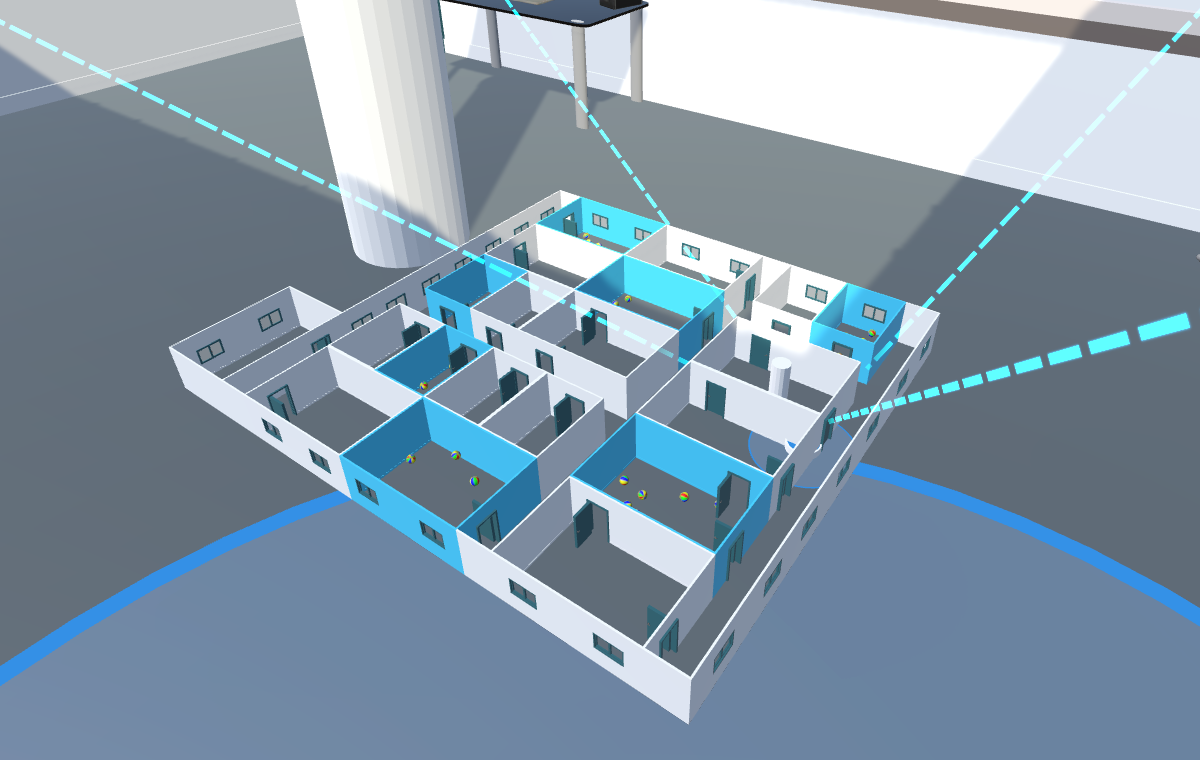
\includegraphics[width=\linewidth]{figures/screenshots/condition_3d_l_x}
    \caption{Beispiel des finalen Megamap-Prototyps in der Übersicht.}
    \label{fig:megamap_overview}
\end{figure}

\section{Unity Engine}
\emph{Unity} \autocite{UnityTechnologies2018} ist eine \emph{Engine} zum Entwickeln von 2D- und 3D-Anwendung (vorwiegend Spiele).
Da Unity plattformunabhängig ist werden die Applikationen gleichzeitig für mehrere Plattformen entwickelt.
Erstellt werden die Anwendungen mit dem Unity Editor.

Eine Unity-Anwendung ist in Szenen unterteilt.
Jede Szene besitzt einen eigenen Szenengraph.
Dieser Graph verwaltet alle Objekte einer Szene.
Unity verwendet ein Entitäten-Komponenten-System.
Das heißt, alle Unity-Objekte sind im Kern attribut- und funktionslose Entitäten (in Unity \emph{GameObject}s genannt).
Die eigentliche Funktionalität wird erst durch Hinzufügen von Komponenten (\emph{Components}) zu den GameObjects deutlich.
Beispielsweise verfügt das GameObject eines Würfel-Objekts über die Komponenten \lstinline{Transform} (Position, Rotation und Skalierung), \lstinline{MeshRenderer} (Geometrie) und \lstinline{BoxCollider} (Kollision).
Neben Anwendungen für den Desktop oder mobile Endgeräte bietet Unity native Unterstützung für eine Vielzahl an AR- und VR-Plattformen an \parencite{UnityTechnologies2018b}.

Zusätzlich zu diesen vorgefertigten Komponenten können auch Skript-Komponenten zu den GameObjects hinzugefügt werden.
Dies ermöglicht Entwicklern, komplett neues Verhalten für Objekte in die Engine zu integrieren.
Die Skripte werden in C\# oder einem Javascript-Dialekt geschrieben.
Die Skripte erben von der Unity-Klasse \lstinline|MonoBehaviour|, wodurch sie in den Lebenszyklus von Unity-Objekten aufgenommen werden und Eventmethoden wie z.\,B. \lstinline|Start()|, \lstinline|Update()|, \lstinline|FixedUpdate()| usw. erhalten \parencite{UnityTechnologies2018c}.

Eine Besonderheit bei Unity im Vergleich zu anderen Engines sind die \emph{Prefabs}.
Dabei handelt es sich um abgespeicherte Konfigurationen von GameObjects inklusive derer Komponenten.
Die Prefabs können dann jederzeit als vorkonfiguriertes Objekt instanziiert werden.
Darüber hinaus lässt sich Unity durch das Importieren von Plugins erweitern.
So werden \emph{Assets} (Texturen, Fonts, Musik, Materialien, Skripte) und Prefabs von anderen Entwicklern in das aktuelle Projekt übernommen.
Aufgrund der einfach zu nutzenden AR-/VR-Funktionalität sowie der Erweiterbarkeit wird Unity für diese Arbeit eingesetzt.

\section{SteamVR Plugin}
Für diese Arbeit wird das \emph{SteamVR Plugin} \autocite{ValveCorporation2018} eingesetzt.
Dieses baut die in Unity integrierte AR-/VR-Unterstützung weiter aus.
Eine zentrale Rolle nimmt das \emph{Player}-Prefab ein.
Durch Platzieren dieses Prefabs in der Unity-Szene werden automatisch GameObjects erzeugt, welche die Positionen und Rotationen vom HMD und Controllern des verbundenen VR-Systems tracken.
Die Zuordnung der Geräte zu den GameObjects ist hardware-übergreifend und geschieht automatisch.
Zudem wird den Nutzern eine Begrenzung des Spielebereichs angezeigt, welcher in diesem Fall durch den Messbereich der stationären Vive Basisstationen gegeben ist.
Ebenso werden 3D-Modelle der Controller und Hände angezeigt, wobei sich die virtuellen Finger während der Controller-Nutzung mitbewegen.
Das Prefab übernimmt außerdem das stereoskopische Rendern, sodass auf dem HMD für jedes Auge ein anderes Bild angezeigt wird, wodurch der Eindruck von räumlicher Tiefe entsteht.

Für diese Arbeit wird außerdem das \lstinline{Interactable}-SteamVR-Skript verwendet.
Über dieses Skript können GameObjects mit einer \lstinline{Collider}-Komponente auf die virtuellen Hände bzw. Controller reagieren und interaktiv gemacht werden (z.\,B. Aufnehmen und werfen von Objekten, anklicken von Knöpfen etc.).
Die Verwendungen dieses Skripts für den Megamap-Prototyp werden an entsprechender Stelle in den folgenden Abschnitten näher beschrieben.

\section{Virtuelle Laborumgebung}
Wie eingangs in \autoref{sec:motivation_ziel} erwähnt war die ursprüngliche Idee dieser Arbeit die Implementierung eines Megamap-Prototyp für das MR-HMD Magic Leap One.
Dabei sollte die virtuelle Karte mithilfe des HMDs in die reale Umgebung des Nutzers integriert werden.

Zu Beginn der Arbeit war allerdings statt der MR-Hardware nur ein Software-Simulator als Entwicklervorschau verfügbar.
Im Verlauf der Arbeit wurde die MR-Hardware veröffentlicht.
Das HMD war in der Arbeitsgruppe Human-Computer~Interaction der Universität Bremen jedoch weiterhin nicht verfügbar.
Daher wurde in dieser Arbeit ein alternativer Prototyp für das VR-HMD HTC Vive entwickelt.
Wie die meisten VR-HMDs verdeckt die Vive das Sichtfeld der Nutzer komplett, um stattdessen die virtuellen Inhalte anzuzeigen.
Somit ist die reale Welt für die Nutzer nicht mehr sichtbar, was die visuelle Integration der Megamap in die reale Umgebung unmöglich macht.

Der entwickelte Prototyp umgeht dieses Problem, indem ein virtuelles Modell der Umgebung im Maßstab 1:1 verwendet wird.
Die reale Welt wird dadurch virtuell simuliert.
Die Megamap kann dann in die \textit{virtuelle} Umgebung des Nutzers integriert werden.
Die Idee hinter diesem Ansatz ist, dass durch die Ähnlichkeit der realen und der virtuellen Umgebung das Prinzip des VR-Prototyps auf ein Szenario mit einem MR-HMD übertragbar ist.
In zukünftigen Arbeiten könnte damit der Megamap-Prototyp auf MR-HMDs eingesetzt werden, ohne grundlegende Änderungen vornehmen zu müssen.

Wie auch die HoloLens erstellt die Magic Leap One durch aktives Tracking der Umwelt intern ein 3D-Modell der Umgebung.
Dieses wird für die Kollisionsberechnung mit den virtuellen Inhalten verwendet.
So können virtuelle Objekte mit realen Gegenständen interagieren (z.\,B. läuft ein Charakter über einen realen Tisch oder ein virtueller Bildschirm wird an einer realen Wand platziert).
Da im Megamap-Prototyp ein 3D-Modell als Umgebung dient, ist die Interaktion von virtuellen Objekten mit der Umwelt implizit möglich.

\begin{figure}[b!]
    \begin{subfigure}{0.5\textwidth}
        \centering
        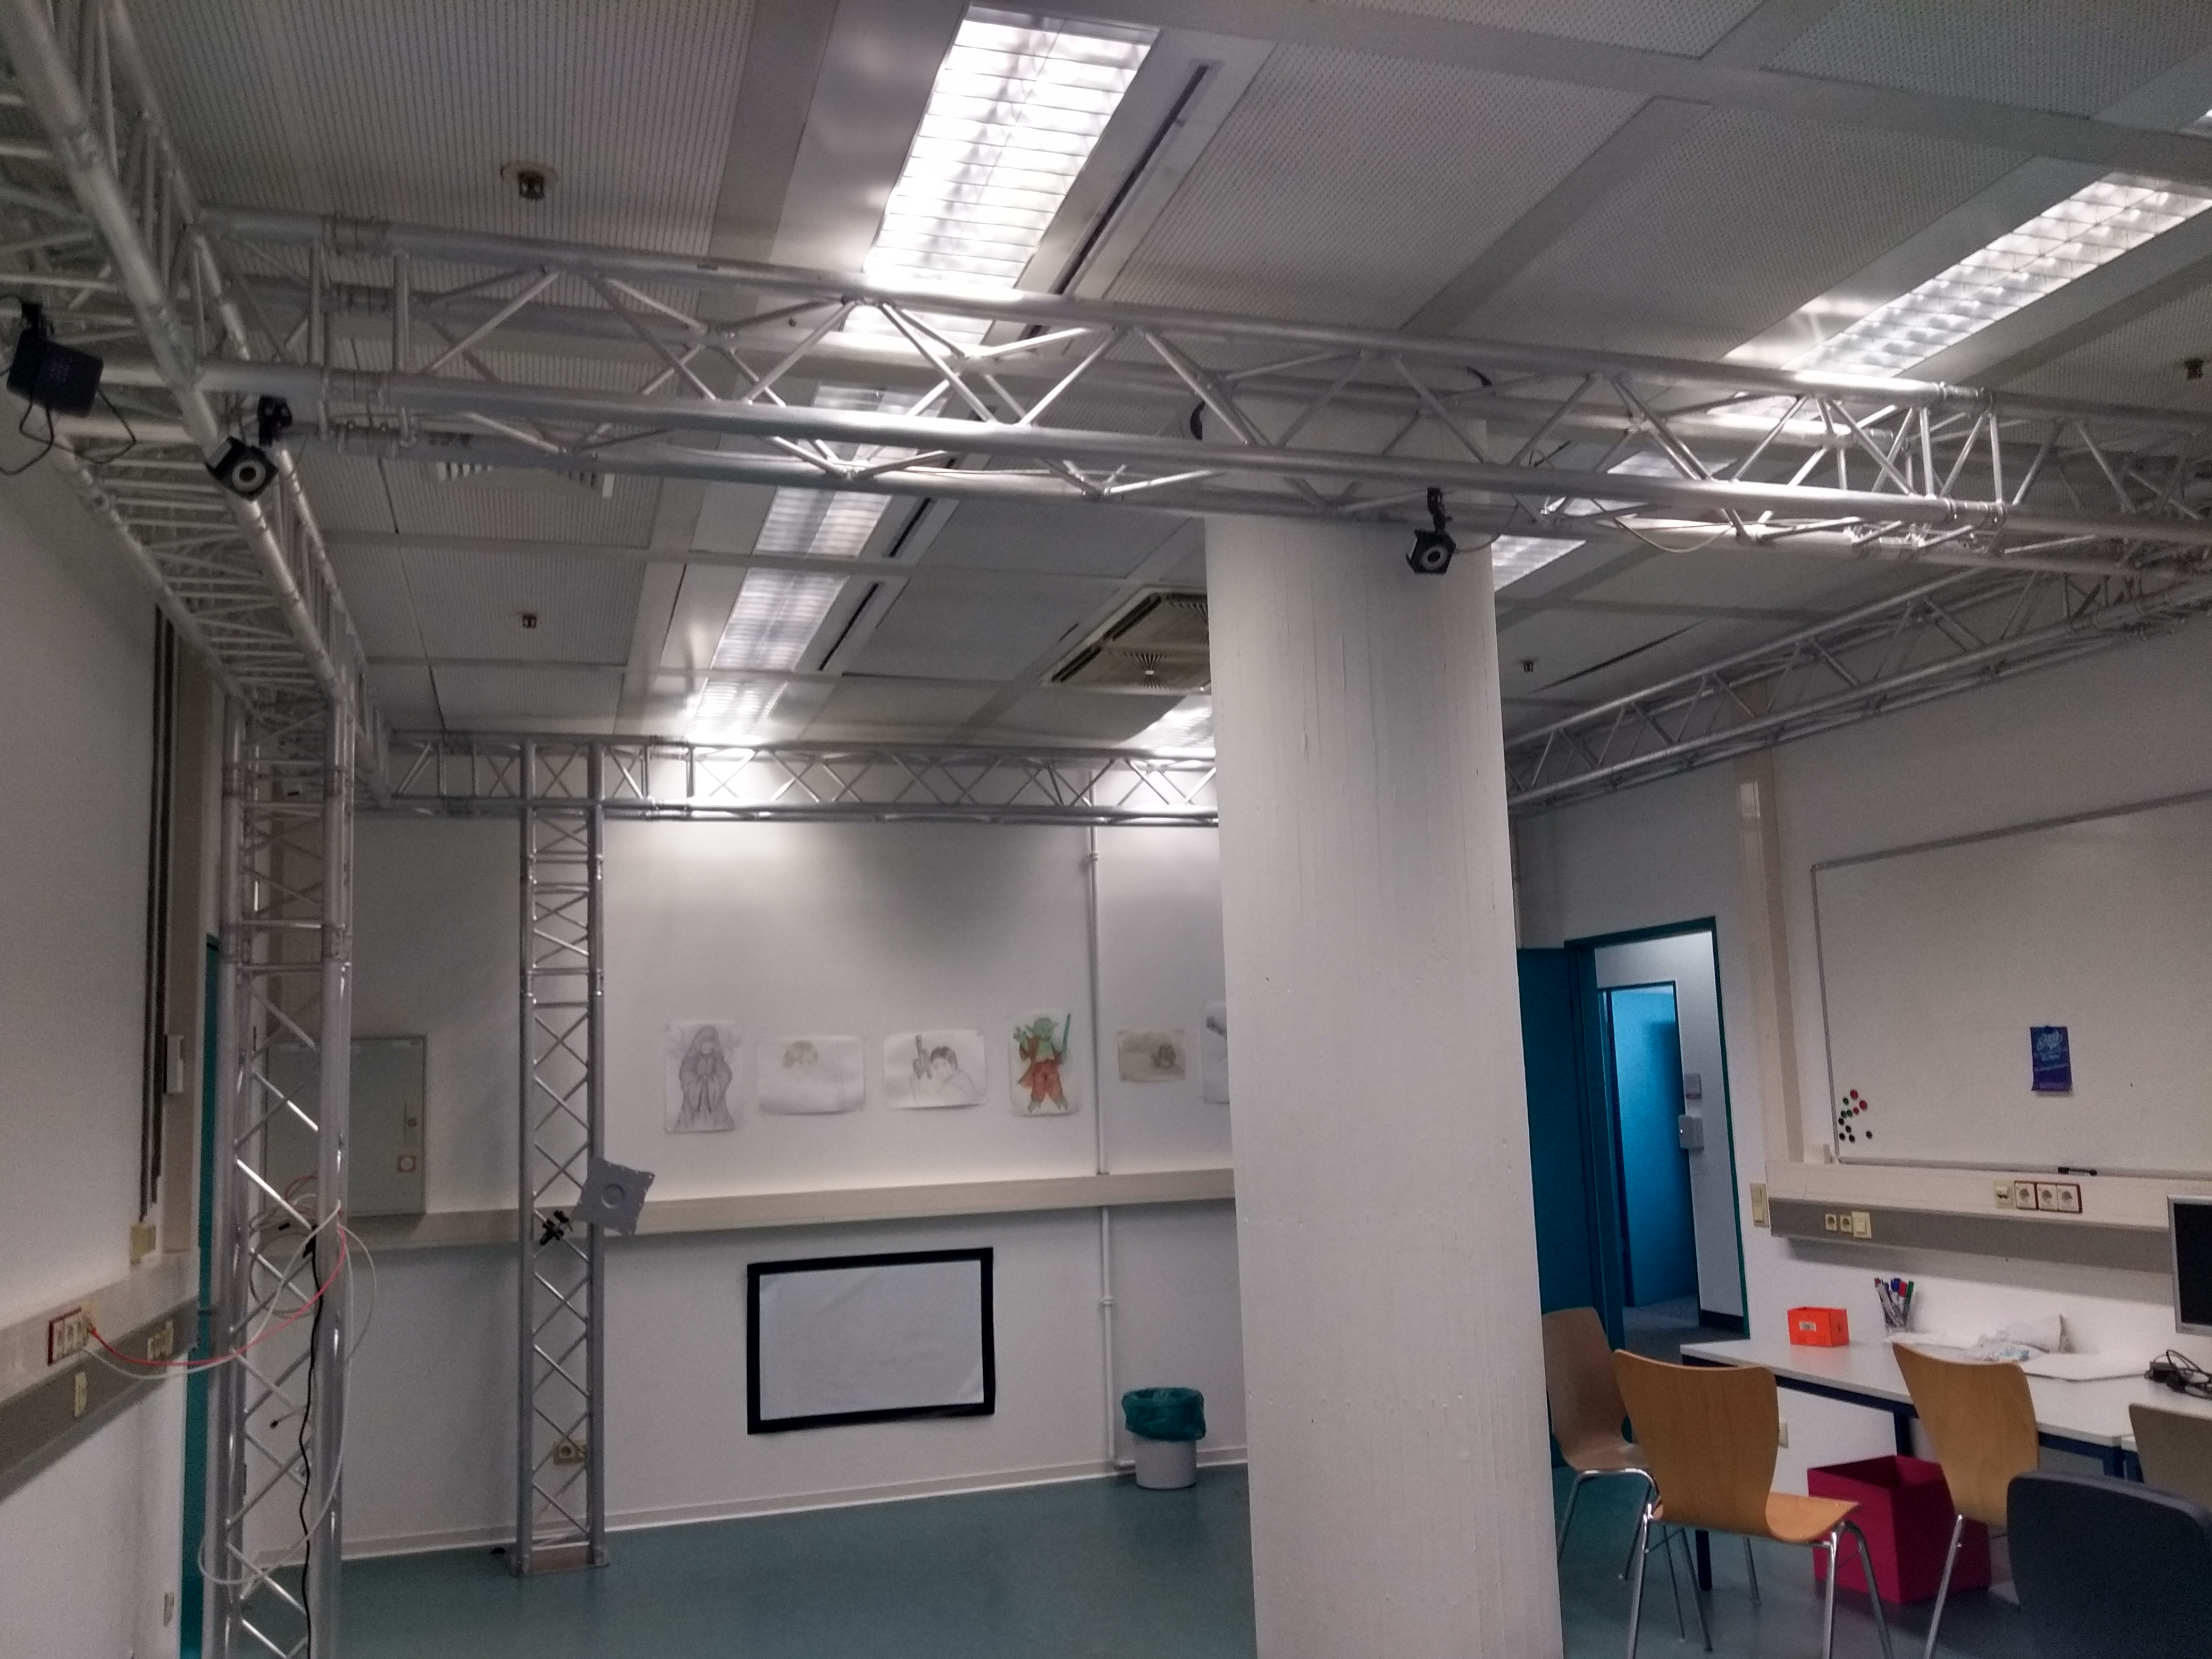
\includegraphics[width=\textwidth, height=4.2cm]{figures/photo_lab}
        \label{sfig:lab_photo}
    \end{subfigure}%
    \begin{subfigure}{0.5\textwidth}
        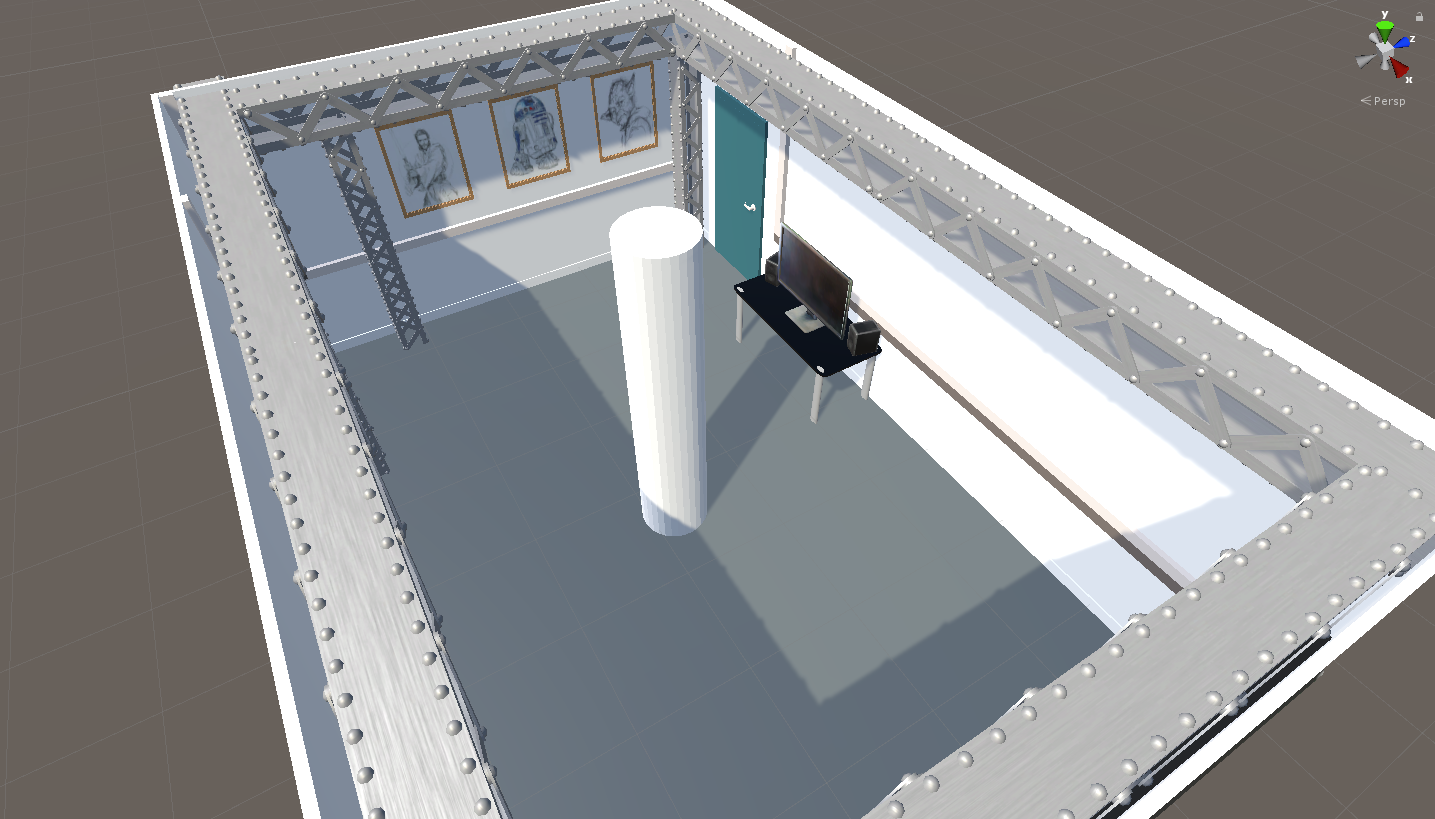
\includegraphics[width=\textwidth]{figures/lab3}
        \label{sfig:lab_screenshot_1}
    \end{subfigure}%
    
    \vspace{-1.25em}
    
    \begin{subfigure}{0.5\textwidth}
        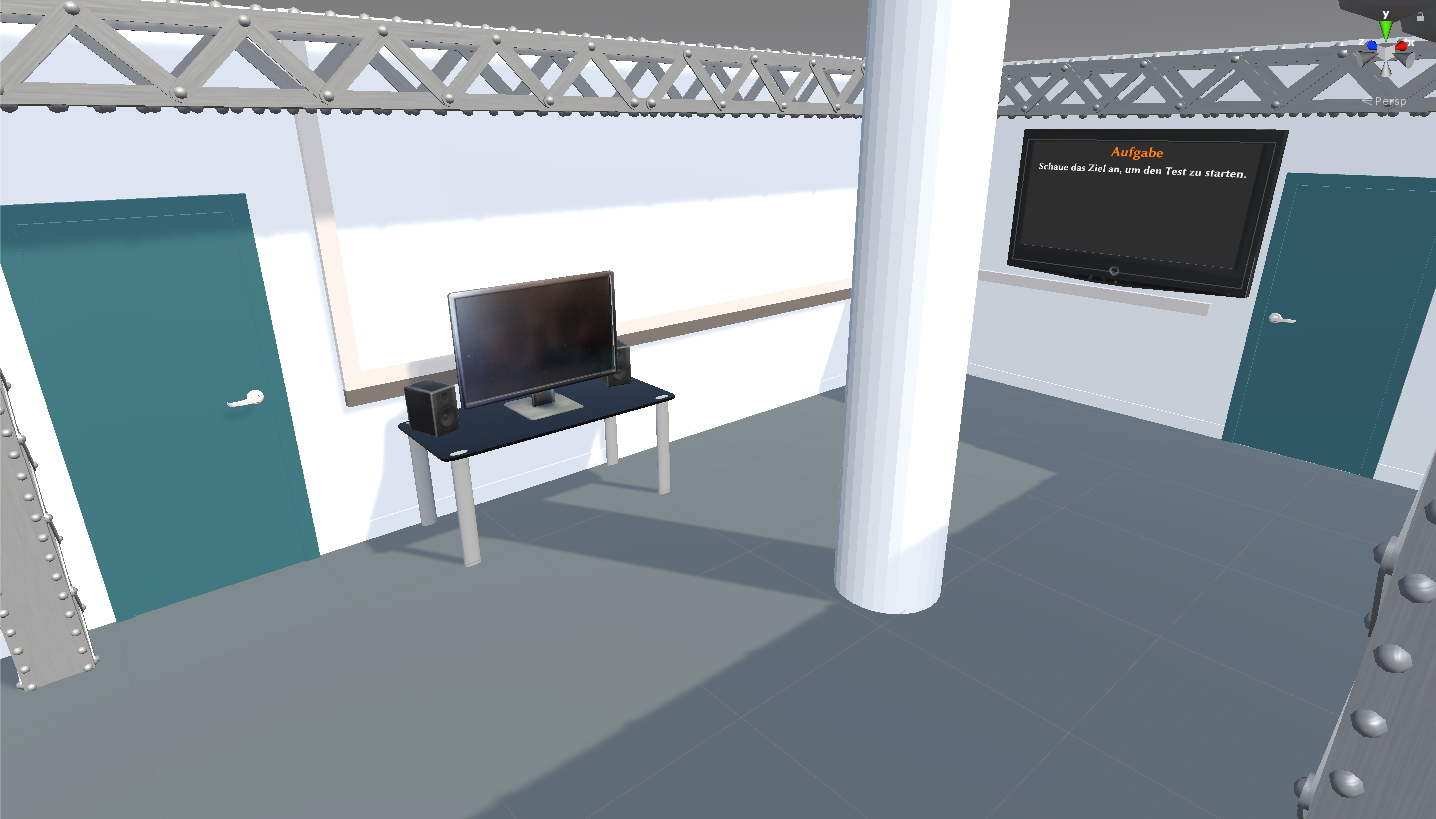
\includegraphics[width=\textwidth]{figures/lab1}
        \label{sfig:lab_screenshot_2}
    \end{subfigure}%
    \begin{subfigure}{0.5\textwidth}
        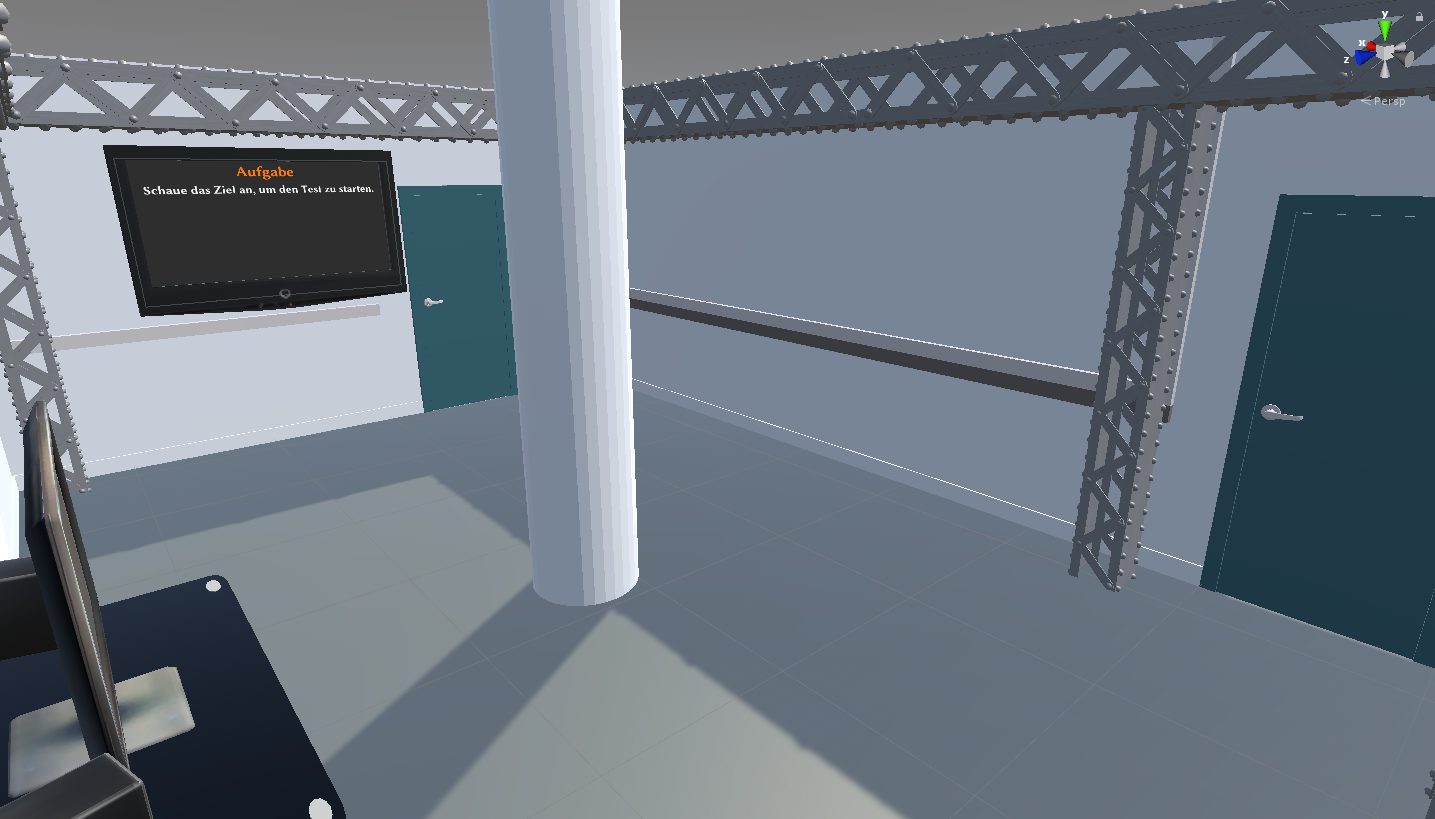
\includegraphics[width=\textwidth]{figures/lab2}
        \label{sfig:lab_screenshot_3}
    \end{subfigure}
    \caption{Um die Situation der MR-Anwendung in VR nachzubilden, wurde der Laborraum im Maßstab 1:1 modelliert. %
        Die Bilder zeigen das Foto des realen Labors (oben links) sowie Screenshots des virtuellen Labors in Unity.}
    \label{fig:lab_environment}
\end{figure}

Für den Prototyp wurde ein maßstabsgetreues 3D-Modell des Laborraums der Arbeitsgruppe Human-Computer~Interaction der Universität Bremen angefertigt, welcher der Durchführungsort der Nutzerstudie ist (siehe \autoref{chap:evaluation}).
\autoref{fig:lab_environment} zeigt ein Foto des Laborraums sowie Screenshots der entsprechenden virtuellen Umgebung.
Der Grundriss des Raums wurde im Modellierungsprogramm \emph{Blender} mithilfe des eingebauten \emph{Archimesh}-Werkzeugs zentimetergenau erstellt.
Das Modell wurde als \texttt{.fbx} in Unity importiert und mit diversen virtuellen Requisiten ergänzt, um den Raum realistischer und dem Original ähnlicher wirken zu lassen.

\subsection*{Synchronisation der realen und virtuellen Position}
Damit die virtuelle Umgebung als Ersatz für die reale Umgebung verwendet werden kann muss sichergestellt werden, dass die Rotation des virtuellen Raums der des realen Raums entspricht.
Außerdem müssen die Positionen der Nutzer zwischen der virtuellen und realen Welt übereinstimmen.
Der Prototyp muss dafür vorab in zwei Schritten konfiguriert werden:

\paragraph{Erster Schritt:}
Während der Kalibrierung der Vive legen die Nutzer den Spielebereich (die sogenannte \emph{Play Area}) fest.
Dies ist der Bereich, in dem sich keine Hindernisse befinden und der für die Basisstationen sichtbar ist.
Hierfür ziehen die Nutzer mit den Controllern ein Rechteck nach, welches dann als Spielebereich gesetzt wird.
Zu beachten ist, dass die längere Seite des Rechtecks orthogonal zur Ausgangsrotation des \lstinline{Player}-Objekts in Unity verläuft.
Die aktuell getrackte Rotation des HMDs wird relativ zur Ausrichtung der Play Area gemessen.
Da SteamVR automatisch die längeren Seiten der Play Area als Vorder- bzw. Rückseite betrachtet, müssen diese orthogonal zur Blickrichtung des \lstinline{Player}-Objekts verlaufen.
Im Fall des entwickelten Prototyps bedeutet dies, dass die Vorderseite der Play Area parallel zu der Wand des Labors verlaufen muss, an der sich die Eingangstür und Tische befinden (siehe \autoref{fig:lab_environment}).
Die korrekte Kalibrierung der Play Area wird in \autoref{fig:ve_setup_correct} skizziert.
Wenn bei der Kalibrierung der Play Area eine andere Ausrichtung gewählt wird als die Ausgangsrotation des \lstinline{Player}-Objekts, weicht die virtuelle Rotation der Nutzer von der realen Rotation im Bezug zum Raum ab.
Effektiv hätte die virtuelle Umgebung dann eine andere Ausrichtung als die reale Umgebung.
Die falsche Kalibrierung wird in \autoref{fig:ve_setup_wrong} dargestellt.

\begin{figure}[hbt]
    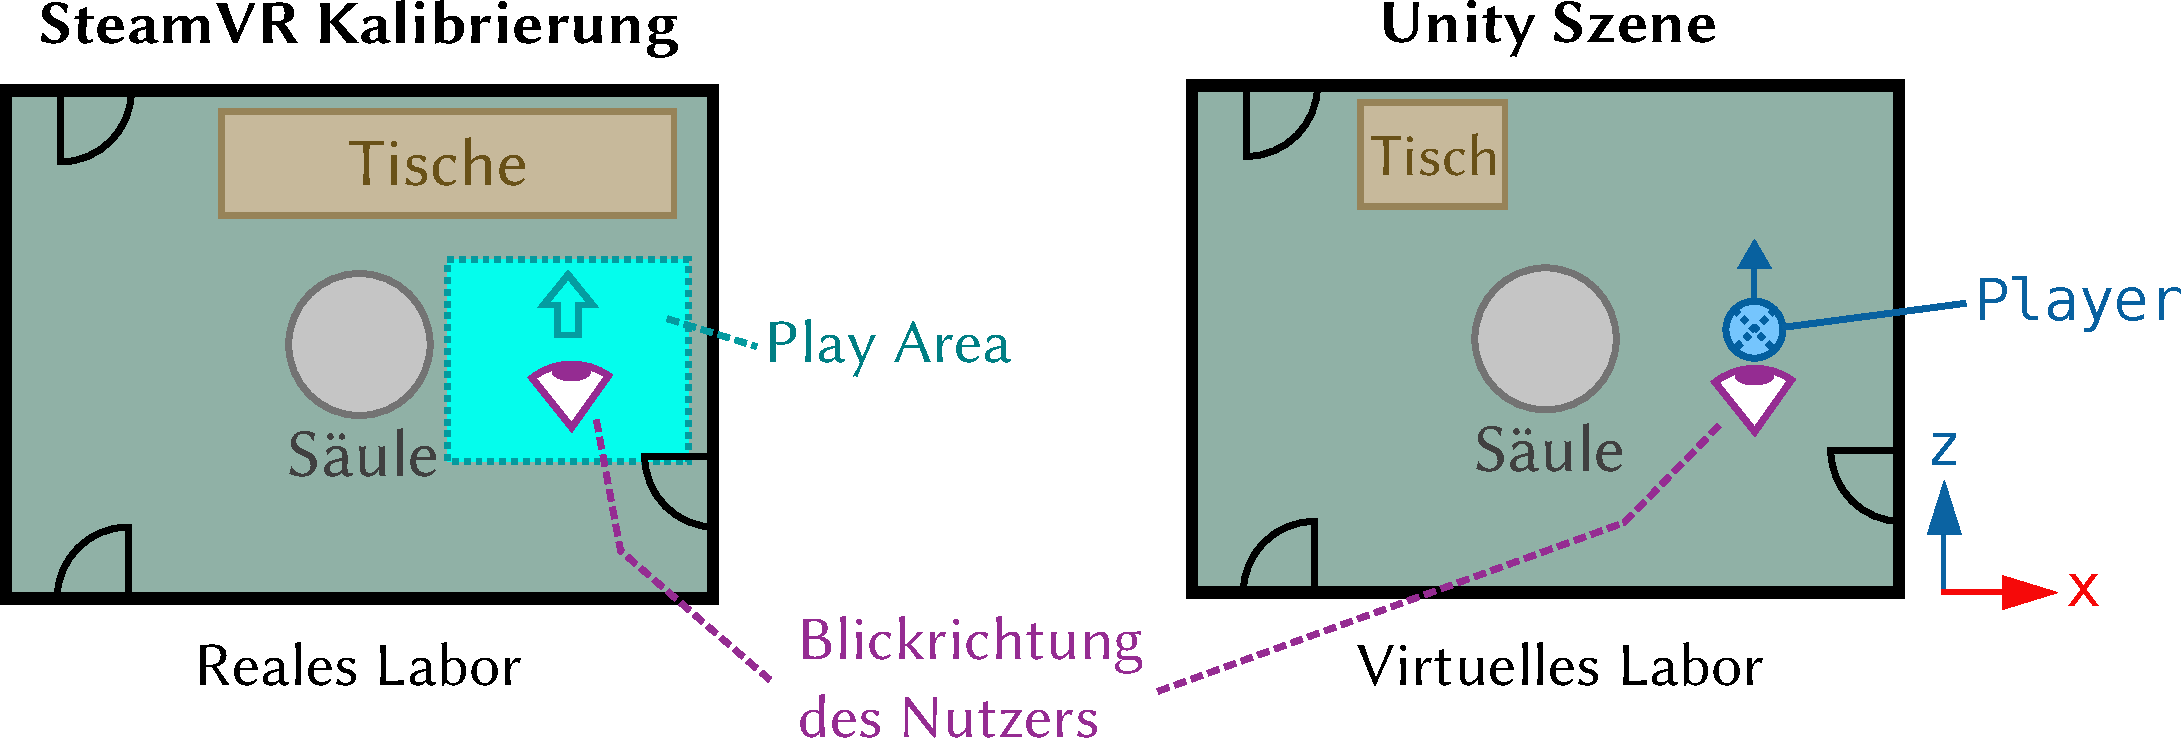
\includegraphics[width=\textwidth]{figures/environment_setup_correct}
    \caption{Die Play Area hat die gleiche Ausrichtung wie das \lstinline{Player}-Objekt in der Grundrotation (entlang z-Achse). %
        Die Rotation des Nutzers in der realen und virtuellen Welt stimmt überein.}
    \label{fig:ve_setup_correct}
\end{figure}
\begin{figure}[hbt]
    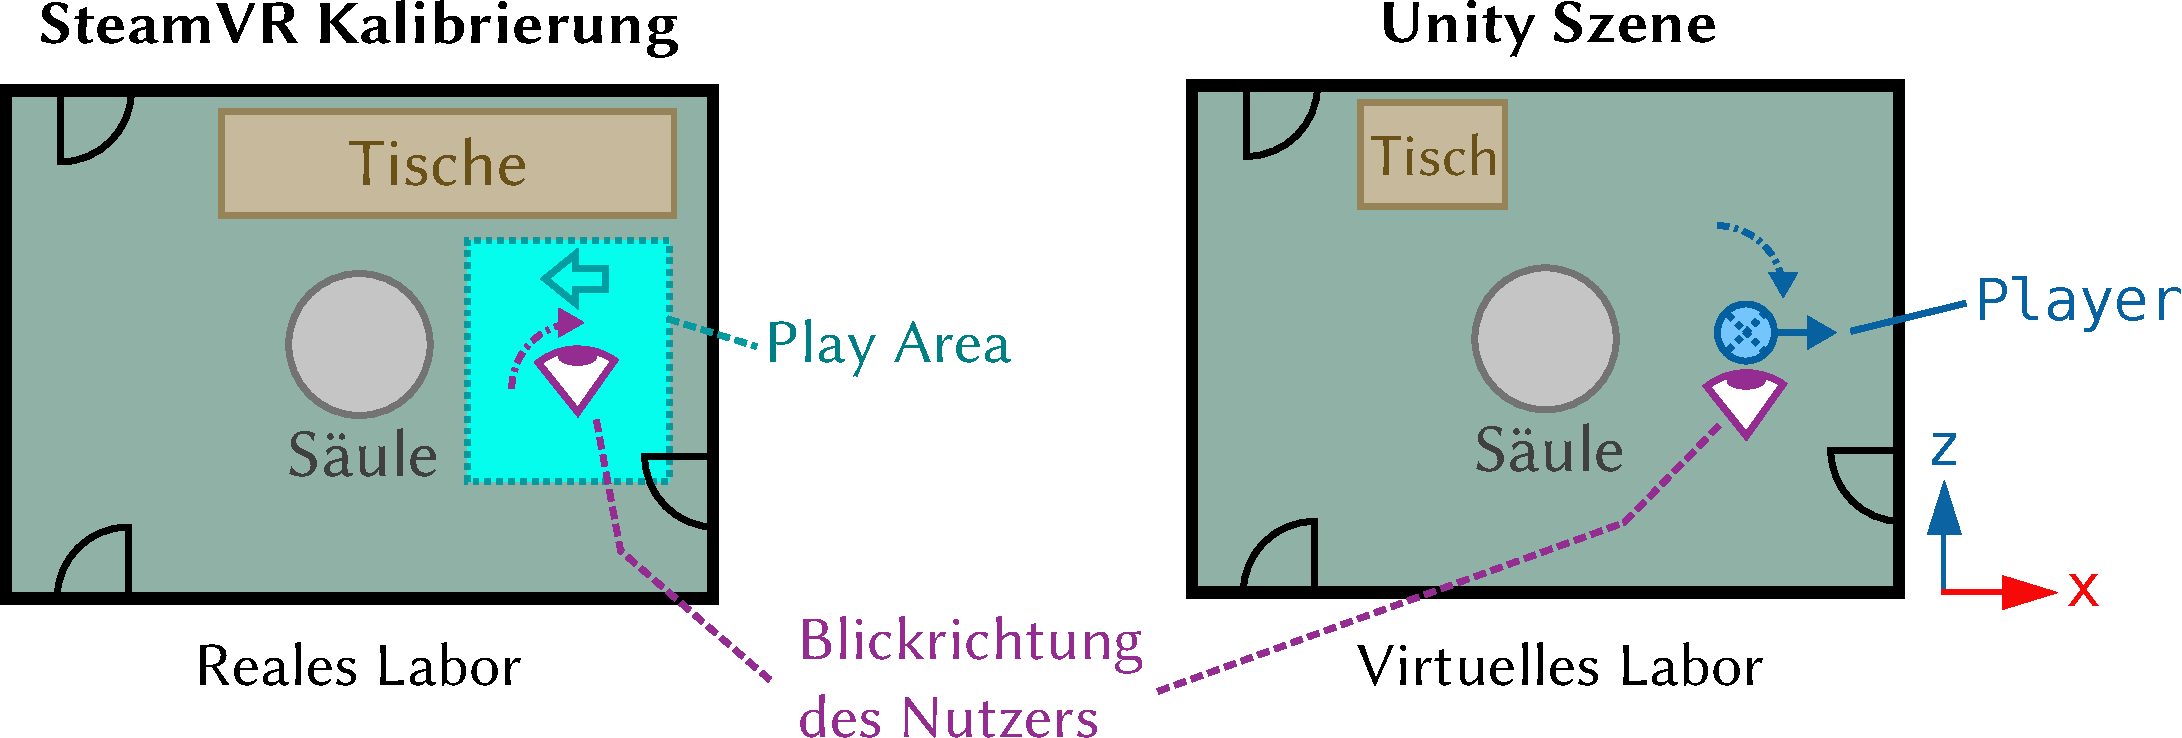
\includegraphics[width=\textwidth]{figures/environment_setup_wrong}
    \caption{Die Play Area hat \emph{nicht} die gleiche Ausrichtung wie das \lstinline{Player}-Objekt in der Grundrotation. %
        Der Nutzer hat einen Rotationsoffset (hier \ang[detect-weight=true]{90}), wodurch für den Nutzer effektiv die Räume unterschiedlich rotiert wirken.}
    \label{fig:ve_setup_wrong}
\end{figure}

Ginge es nur um den visuellen Reiz in der virtuellen Umgebung, würden die Nutzer diese Abweichung lediglich beim Aufsetzen des HMDs bemerken (da dann der virtuelle Raum anders rotiert wäre als der reale).
Wenn aber zum Beispiel der Tastsinn eine Rolle spielt, ist eine korrekte Ausrichtung des virtuellen Raums sinnvoll.
Da in dem entwickelten Prototyp nicht ausgeschlossen ist, dass die Nutzer die Play Area verlassen und beispielsweise die Säule oder Wände mit den Händen berühren, ist es für die Immersion von Vorteil, wenn das Berühren der virtuellen Objekte mit den taktilen Reizen der realen Objekte verknüpft wird.
Weiterhin wird durch die korrekte Ausrichtung die Messung des Abweichungsfehlers (siehe \autoref{chap:evaluation}) beim Zeigen auf Objekte erleichtert.

\paragraph{Zweiter Schritt:}
Neben der Orientierung der Nutzer muss die Position des virtuellen Raums angepasst werden, wenn dieser die reale Umgebung bestmöglich überlagern soll.
Dies resultiert (wie bei der Rotation) aus der Tatsache, dass die getrackte Position des HMDs relativ zur Play Area gemessen wird, welche sich durch den Kalibrierungsvorgang von SteamVR ändern kann.
Um die neue Position des virtuellen Raums zu bestimmen wird für den Prototyp wie folgt vorgegangen:

Der Prototyp wird mit seiner Ausgangsposition im Unity Editor ausgeführt.
Die Ecke \enquote{links unten} aus Vogelperspektive des virtuellen Labors befindet sich an der Unity-Welt-Koordinate $(0, 0, 0)$.
Die Controller, welche im HMD durch 3D-Modelle visualisiert sind, werden in den Ecken des virtuellen Raums platziert.
Dabei wird darauf geachtet, dass sie von den Basisstationen weiterhin erkannt werden.
Nun wird im realen Labor die Entfernung von den Controllern zu den entsprechenden Ecken des Raums gemessen, was der Abweichung der virtuellen zur realen Welt entspricht.
Die Entfernungen werden gemittelt.
Der resultierende Offset wird dann im Unity Editor verwendet, um das virtuelle Labor zu verschieben.
Dieser Offset ist nun solange gültig, bis die Play Area neu kalibriert wird.
Wie auch schon bei der Rotation ist diese Angleichung erst dann für die Nutzer bemerkbar, wenn sie versuchen physische Objekte wie Wände oder die Säule zu berühren.
Würde die Verschiebung des Raums nicht durchgeführt werden, könnten Nutzer mit den Controllern durch die virtuellen Objekte hindurch greifen oder sie würden auf physische Barrieren stoßen, obwohl die virtuellen Objekte noch weiter entfernt sind.
Nach diesen beiden Schritten kann der virtuelle Raum als Ersatz für die reale Umgebung verwendet werden, die in einer MR-Anwendung ohne vorheriges Modellieren verfügbar wäre.

\section{Das Megamap-GameObject}
\begin{figure}[t]
    \centering
    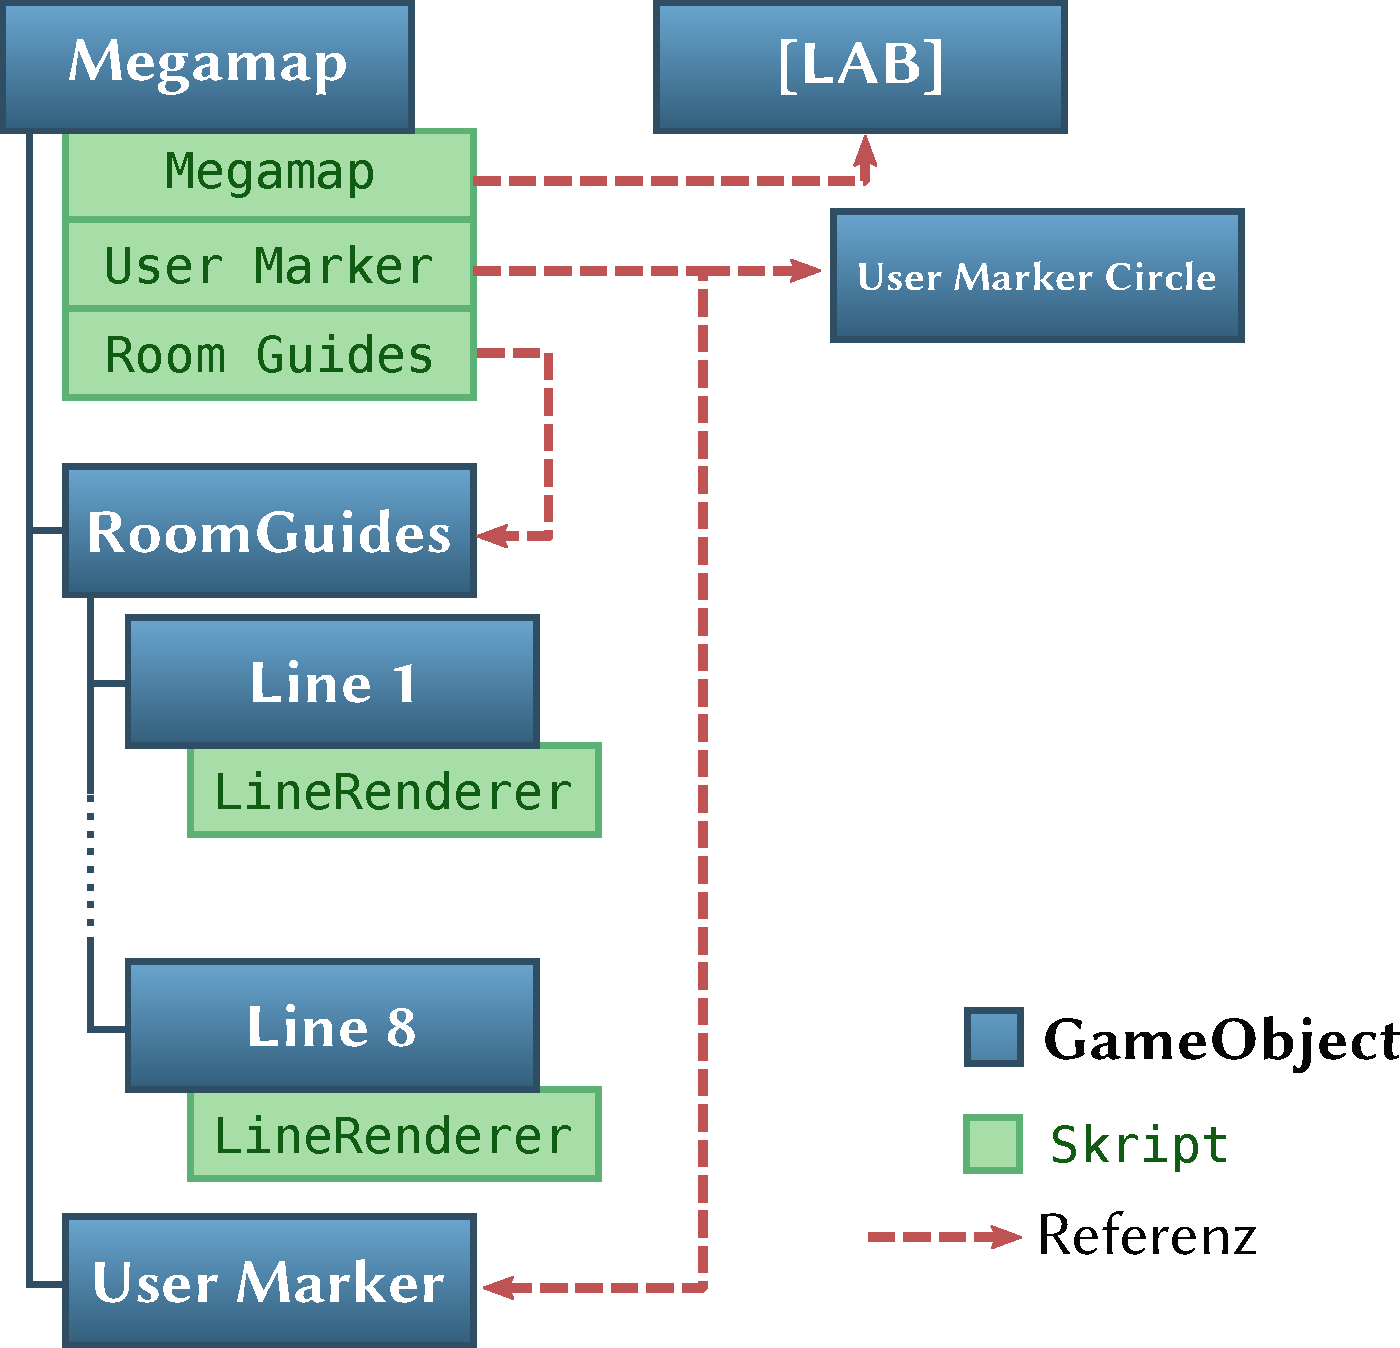
\includegraphics[height=8.5cm]{figures/unity_megamap_object}
    \caption{Übersicht des Megamap-GameObjects.}
    \label{fig:unity_megamap_object}
\end{figure}

Der grundlegende Baustein der Implementierung ist das Megamap-GameObject.
Eine strukturelle Übersicht des Objekts wird in \autoref{fig:unity_megamap_object} gegeben.
Das Objekt setzt sich aus drei Teilen zusammen, die jeweils durch eigene Komponenten repräsentiert werden:

Das Skript \textbf{\lstinline{Megamap}} bietet allgemeine Einstellungsmöglichkeiten zur Darstellung der Megamap.
Es lassen sich z.\,B. die Skalierung oder die Entfernung zum Boden ändern.
Weiterhin bietet das Skript die Methoden \lstinline{Show()} und \lstinline{Hide()}, mit denen die Karte angezeigt bzw. ausgeblendet werden kann.
Falls dabei das Feld \lstinline{useAnimation} auf \lstinline{true} gesetzt ist, wird die Karte beim Anzeigen durch eine Animation von einer 1:1 Raumgröße auf die eingestellte Skalierung nach und nach herunterskaliert (beim Ausblenden analog ein Hochskalieren).
Die Megamap wird standardmäßig Nutzer-zentriert platziert.
Das bedeutet, dass die Nutzer sowohl in der realen Welt als auch auf der Karte die gleiche Position einnehmen.
Hierfür wird die virtuelle Umgebung referenziert und der Abstand vom HMD zum Ursprung des Labor-Modells ermittelt.
Dieser Abstand wird dann wie die Megamap skaliert und die Karte wird um den skalierten Abstand verschoben.
Sowohl die Animation als auch die Zentrierung sollen es den Nutzern erleichtern, ihre eigene Position auf der Karte zu finden.
Außerdem sollen der Bezug vom Laborraum auf der Karte zum umgebenden Laborraum hervorgehoben werden.

Das \lstinline|Megamap|-Skript dient lediglich als Schnittstelle zur Manipulation der Karte.
Das eigentliche 3D-Modell, welches als Karte verwendet wird, ist von diesem Skript unabhängig und wird erst zur Laufzeit durch andere Skripte als aktive Karte gesetzt.
Hierfür bietet das \lstinline|Megamap|-Skript die Methode \lstinline|SetMap(...)| an, welche als Parameter unter anderem eine Referenz auf ein \lstinline|IndoorMap|-Skript erwartet.
Dank dieser Trennung von Schnittstelle und Modell können zur Laufzeit unterschiedliche Indoor-Karten gewechselt werden, was für die Nutzerstudie in \autoref{chap:evaluation} Voraussetzung ist.
Die Details zum \lstinline|IndoorMap|-Skript werden in \autoref{sec:indoor_maps} ausgeführt.

\begin{figure}
    \centering
    \begin{minipage}[t]{.485\textwidth}
        \centering
        \vspace{0pt}
        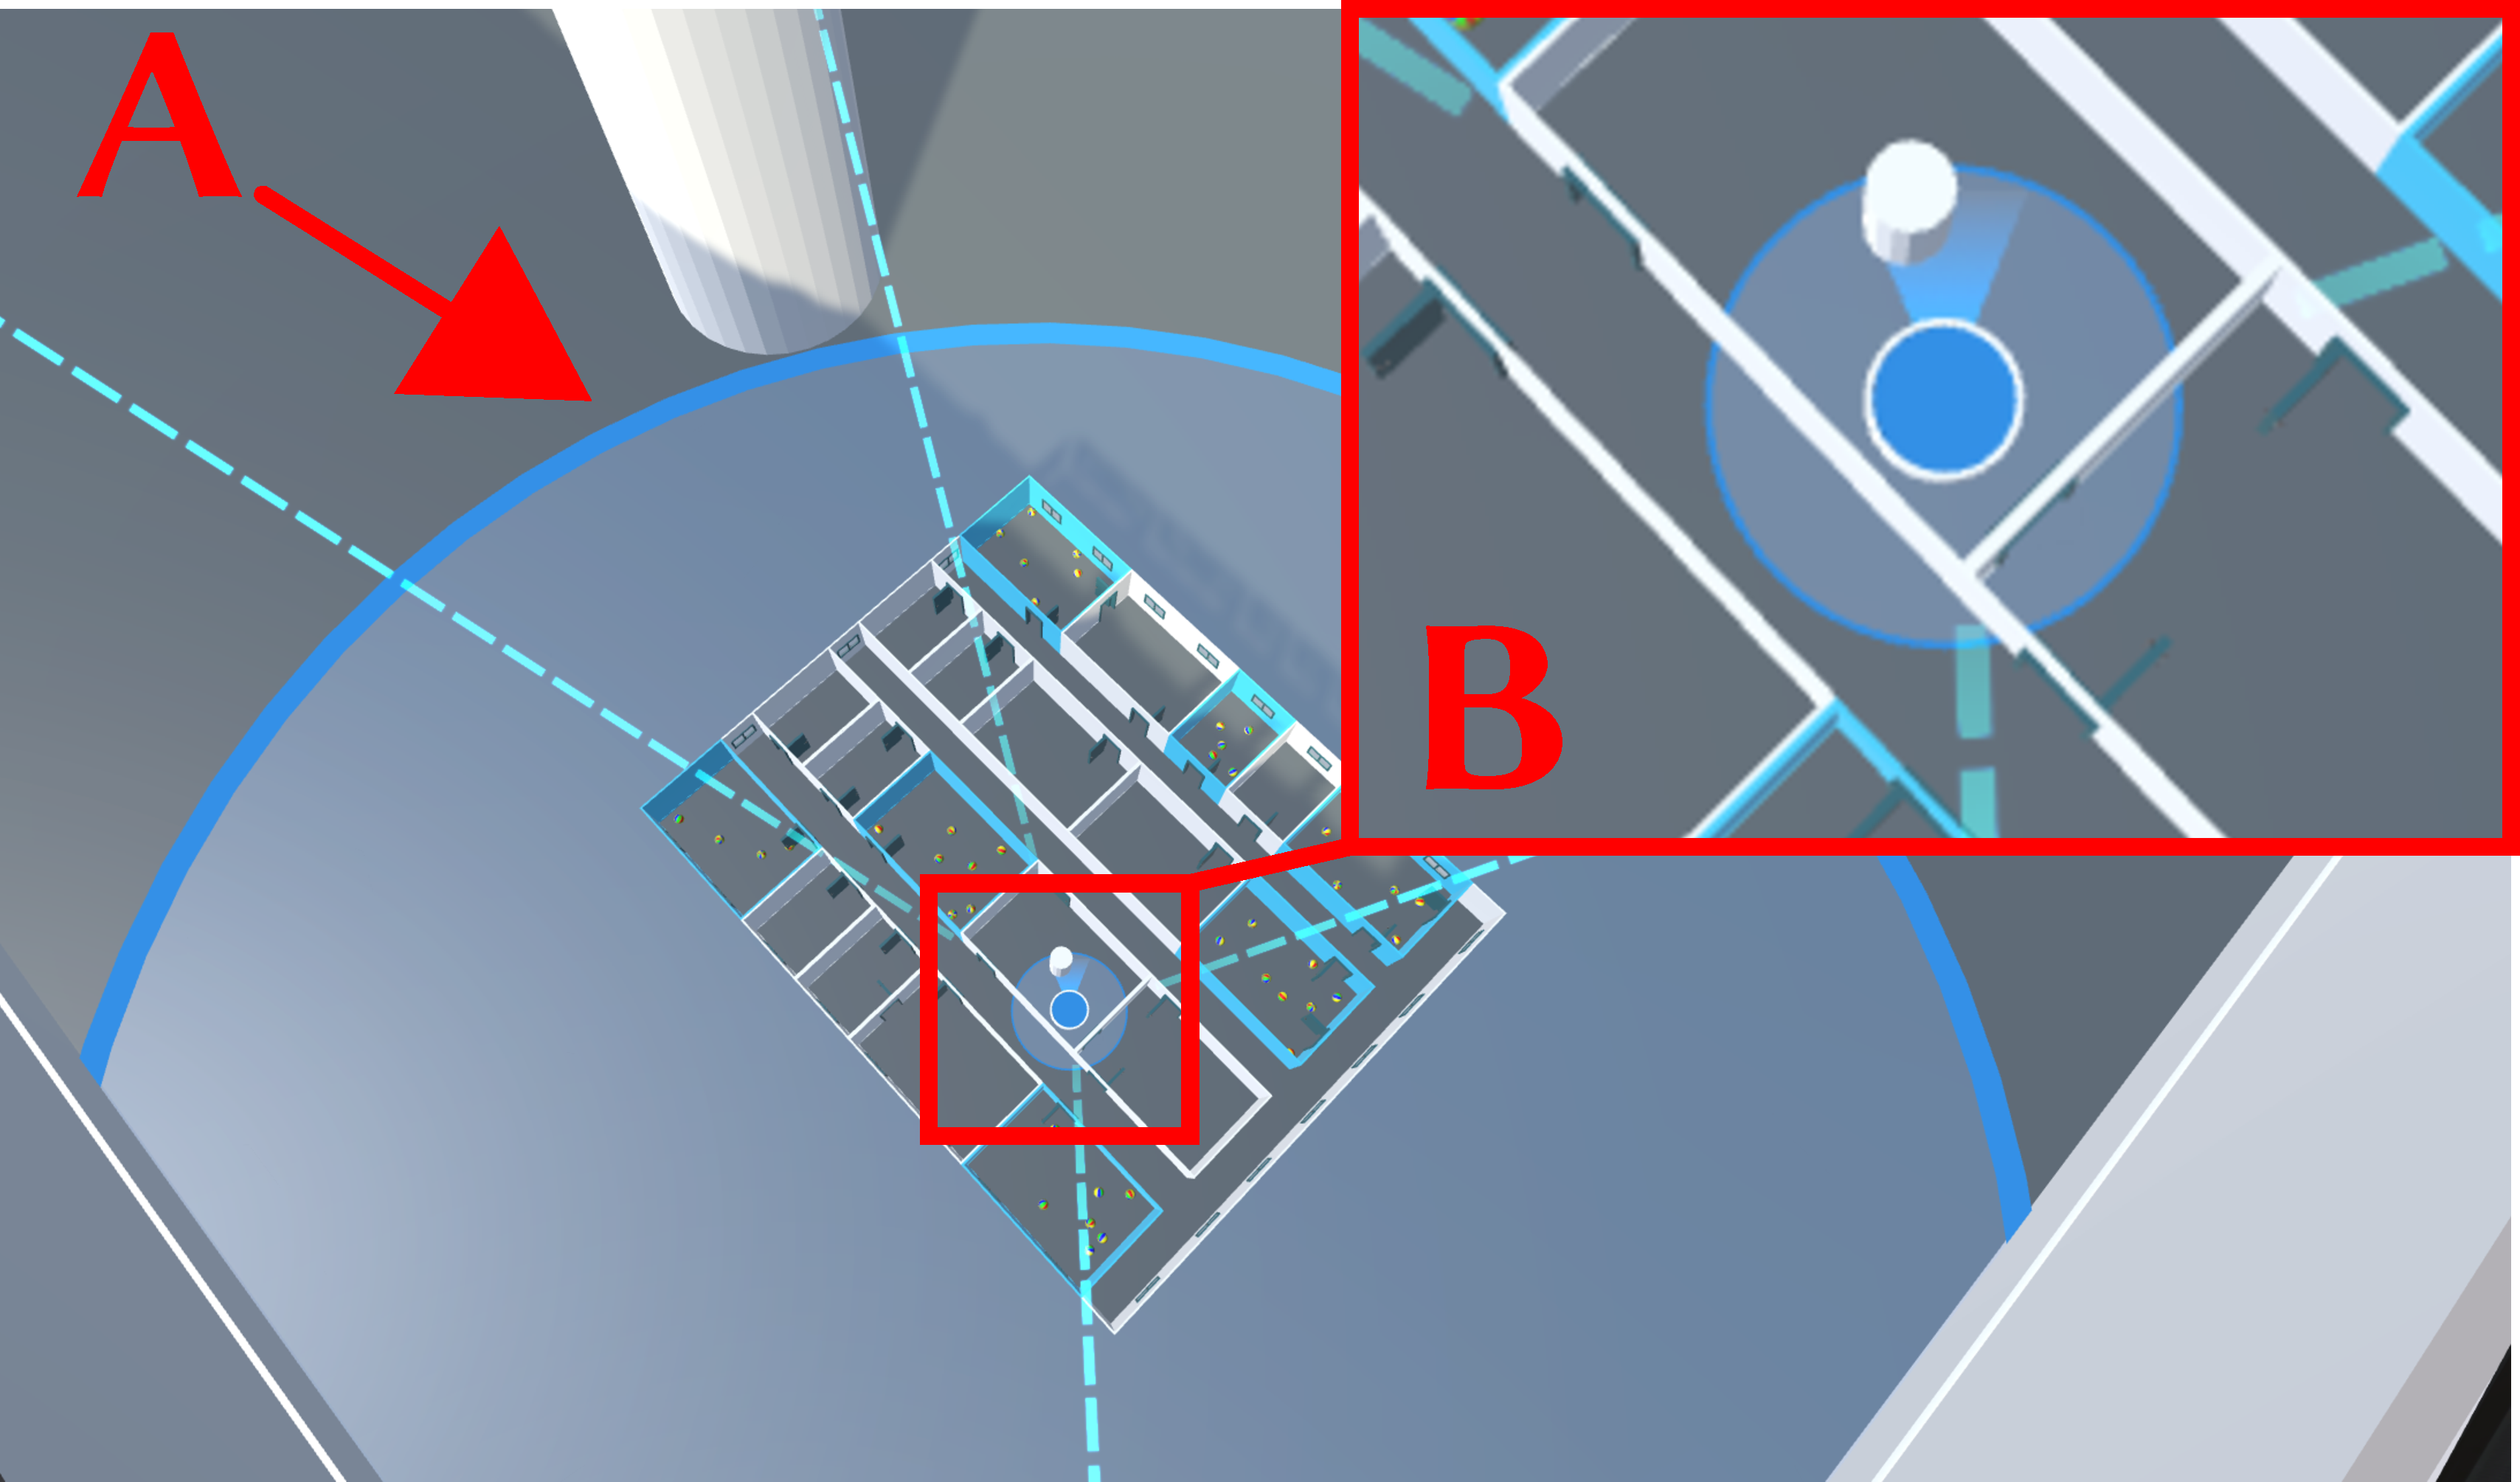
\includegraphics[width=\linewidth]{figures/megamap_user_marker.pdf}
        \captionof{figure}{Der User Marker zeigt die Position der Nutzer auf der Megamap an. %
            \textcolor{red}{A:} Marker in Umgebung. %
            \textcolor{red}{B:} Marker auf Karte.%
        }
        \label{fig:user_marker}
        \vfill
    \end{minipage}
    \hfill
    \begin{minipage}[t]{.485\textwidth}
        \centering
        \vspace{0pt}
        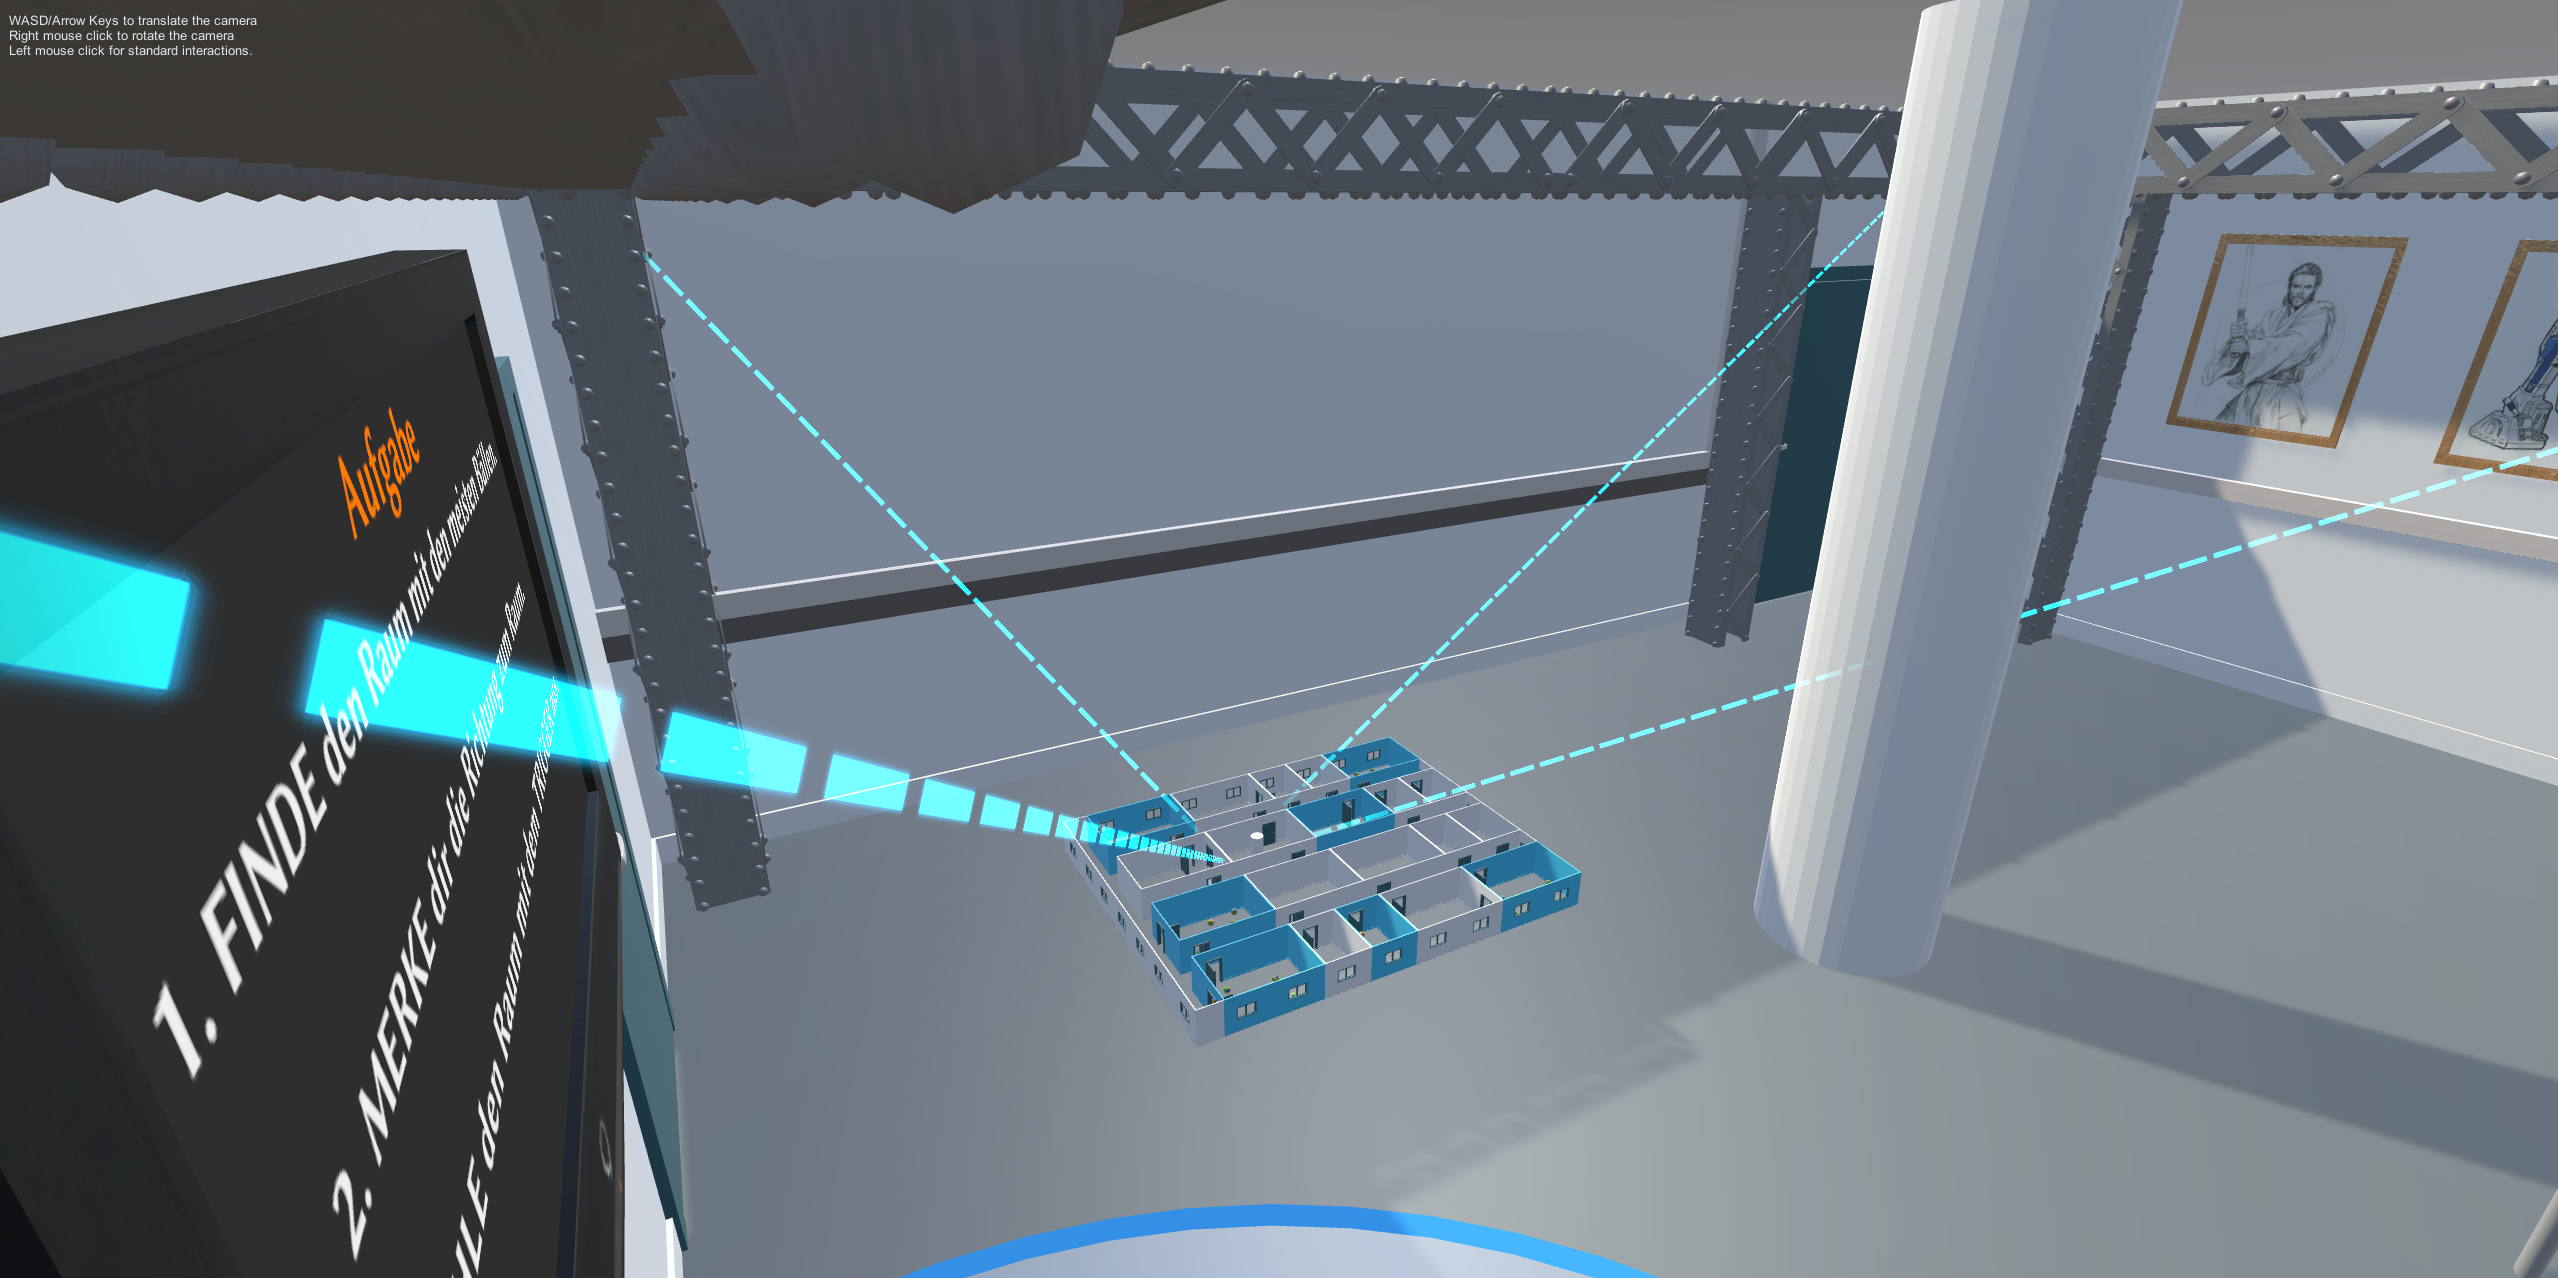
\includegraphics[width=\linewidth, height=4.2cm]{figures/megamap_room_guides}
        \captionof{figure}{Die Room Guides verbinden die Ecken des umgebenden Raums mit dem entsprechenden Raum auf der Megamap.}
        \label{fig:room_guides}
    \end{minipage}
\end{figure}

Der zweite Teil des Megamap-Objekts, das \textbf{\lstinline|User Marker|} Skript, dient ebenfalls der Orientierung für die Nutzer.
Analog zu Kartenanwendungen wie Google Maps befindet sich eine Markierung auf der Megamap, welche die aktuelle Position der Nutzer anzeigt.
Da es sich bei der Megamap um eine dreidimensionale Karte handelt wird hier ein Zylinder in Form ähnlich eines Pucks benutzt (siehe \autoref{fig:user_marker}).
Mittels eines transparenten Kegels wird außerdem die aktuelle Rotation der Nutzer verdeutlicht.
Um den Bezug von der Markierung auf der Karte zur Umgebung zu verstärken ist auch in dieser ein Kreis platziert, welcher auf die Nutzer zentriert ist.

Der dritte Teil des Megamap-Objekts ist das \textbf{\lstinline|Room Guides|} Skript.
Es zeichnet Linien von den Ecken des umgebenden Laborraums zum Laborraum auf der Karte (siehe \autoref{fig:room_guides}).
Die Linien heben den Raum hervor, in dem sich die Nutzer befinden und stellen somit einen Bezug zur Umgebung her.
Implementiert sind diese Führungslinien als acht \lstinline|GameObject|s mit jeweils einer \lstinline|LineRenderer|-Komponente, die zusammen mit der Megamap ein- bzw. ausgeblendet werden.
Für die Startpunkte der Linien (die Ecken des umgebenden Raums) wird über die \lstinline|Renderer|-Komponente des Labor-Modells auf dessen \emph{Bounding Box} zugegriffen.
Die Eckpunkte der Bounding Box sind die Startpunkte der Linien.
Die Endpunkte der Linien werden berechnet, indem die Startpunkte mit der Transformationsmatrix der Megamap multipliziert werden.
So entsteht der Effekt, dass die Linien zu den Eckpunkten des Labors auf der Karte hinführen.
Standardmäßig werden über das Feld \lstinline|showUpperOnly| nur die oberen vier Linien angezeigt, da die unteren Führungslinien vom Rest der Megamap verdeckt werden würden.

\section{Erstellung der Indoor-Karten}
\label{sec:indoor_maps}
Wie bereits erwähnt ist das eigentliche 3D-Modell, welches das Layout des Gebäudes repräsentiert, vom \lstinline|Megamap|-Skript getrennt.
Für den entwickelten Prototyp werden vorab erstellte 3D-Modelle eingesetzt, die in Blender mit dem Archimesh-Werkzeug modelliert wurden.
Die erstellten Karten sind 3D-Modelle, bei denen die einzelnen Räume als separate GameObjects in Unity verfügbar sind.
\autoref{fig:room_hierarchy} zeigt schematisch, wie die Objekthierarchie für die Indoor-Karten in Unity aufgebaut ist.

Für die Nutzerstudie aus \autoref{chap:evaluation} ist es notwendig, dass die Nutzer mit Räumen interagieren können.
Es wird eine Suchaufgabe implementiert, bei der die Nutzer einen spezifischen Raum finden und auswählen müssen.
Die Nutzer können mit den Vive-Controllern Räume anvisieren und durch Betätigung des Triggers auswählen.
Handelt es sich um den gesuchten Raum, wird die Karte ausgeblendet.
Ansonsten wird der Raum als \enquote{falscher Raum} hervorgehoben.

\begin{figure}[tbh]
    \centering
    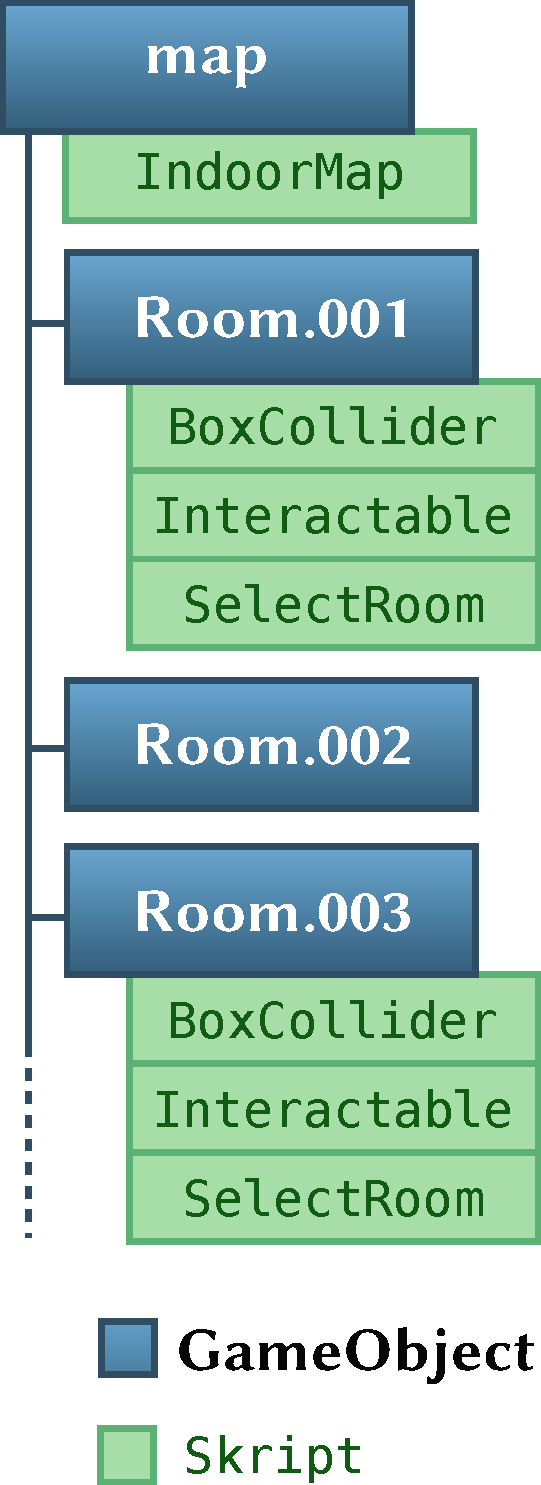
\includegraphics[height=9cm]{figures/unity_indoor_map}
    \caption{Objekthierarchie des IndoorMap-Objekts,}
    \label{fig:room_hierarchy}
\end{figure}

Diese Interaktionsmöglichkeit wird durch das \lstinline|SelectRoom|-Skript umgesetzt.
Das Skript verwendet die SteamVR-Komponente \lstinline|Interactable|, wodurch Räume auf An\-nä\-he\-rungs- und Interaktionsevents der Vive-Controller reagieren können.
Im Skript werden dazu spezielle SteamVR-Methoden implementiert.
Die Methode \lstinline|OnHandHoverBegin(...)| wird ausgelöst, sobald die \lstinline|HoverTransform| des Vive-Controllers den Collider des Raums berührt.
In der Methode wird der Raum gelb hervorgehoben, wenn er zuvor nicht angeklickt wurde.
Wenn er zuvor bereits angeklickt wurde (und nicht der gesuchte Raum ist) wird der Raum stattdessen rot eingefärbt.

Die Methode \lstinline|OnHandHoverEnd(...)| setzt die Farbe des Raums in den Normalzustand zurück, wenn der Vive-Controller den Collider des Raums verlässt.
Somit ist die farbliche Änderung nur sichtbar, solange der Raum mit dem Controller anvisiert wird.

Die \lstinline|HandHoverUpdate(...)|-Methode wird in jeder Update-Iteration von Unity ausgeführt, solange der Vive-Controller den Collider des Raums überlappt.
In der Methode wird überprüft, ob aktuell der Trigger des Controllers betätigt wird.
Sobald der Trigger von den Nutzern gedrückt wird, wird ein Event ausgelöst, was die Auswahl eines Raums signalisiert.
Handelt es sich dabei um den gesuchten Zielraum, wird das Event \lstinline|OnTargetRoomSelected| ausgelöst.
Dieses wird an anderer Stelle benutzt, um die Karte bei Auswahl des Zielraums auszublenden.
Wenn der falsche Raum gewählt wird, wird stattdessen das Event \lstinline|OnWrongRoomSelected| aktiviert.
Dieses wird genutzt, um die Auswahl von falschen Räumen zu zählen und in \autoref{chap:evaluation} auszuwerten. 

Um den Zugriff auf die Räume zu vereinfachen verfügt das IndoorMap-Objekt über das gleichnamige Skript \lstinline|IndoorMap|.
Dieses bietet C\#-Eigenschaften (\emph{Properties}) an, um die Liste aller Räume bzw. die Liste aller \emph{auswählbarer} Räume zu erhalten (\lstinline|Rooms| bzw. \lstinline|SelectableRooms|).

Damit die Megamap das IndoorMap-Objekt als Karte verwendet wird es an die Methode \lstinline|SetMap(...)| des \lstinline|Megamap|-Skripts übergeben.
Hierdurch wird das IndoorMap-Objekt zu einem Kind-Objekt der Megamap.
Die Skalierung und Translation der Megamap werden automatisch für das Kartenmodell übernommen.
Die Karte kann durch weitere Aufrufe von \lstinline|SetMap(...)| ausgetauscht werden.

\section{Interaktion mittels virtuellem Laserpointer}
Mit den \lstinline|SelectRoom|- und \lstinline|Interactable|-Skripten können die Nutzer die Räume auf der Karte mit dem Vive-Controller auswählen.
Allerdings müssten sie sich (ohne weitere Maßnahmen) zu den einzelnen Räumen hinbewegen, um diese mit dem Vive-Controllern zu berühren und auszuwählen.
In informellen Vortests des Prototyps	 zeigte sich, dass die Bewegung zu den Räumen umständlich ist, wenn lediglich ein einzelner Raum gefunden werden soll.
Die Play Area der Vive schränkt die Bewegung der Nutzer zusätzlich ein, da außerhalb der Play Area mit Hindernissen gerechnet werden muss und das Tracking durch die Basisstationen ungenauer wird.

Für den finalen Prototyp wurde daher eine Methode zur entfernten Auswahl von Räumen entwickelt.
Über einen virtuellen \enquote{Laser Pointer} können Nutzer mit den Vive-Controllern auf Räume zeigen und diese mit dem Trigger auswählen.
Der Screenshot in \autoref{fig:laserpointer_screenshot} zeigt ein Beispiel.
Das Skript \lstinline|LaserPointer| setzt dies um, indem es einen \lstinline|LineRenderer| aktiviert, welcher einen Lasterstrahl darstellt.
Der Strahl verläuft vom Controller geradeaus in die Szene.
In der Methode \lstinline|Update()| wird dann durch \lstinline|Physics.RaycastAll(...)| ein Schnitttest zwischen dem Strahl und Collidern in der Szene durchgeführt.
Falls ein Collider vom Strahl getroffen wird und der Collider zu einem der Räume gehört, wird der Schnittpunkt als Endpunkt des Laserstrahls gesetzt.
So entsteht der Effekt, dass der Laserstrahl nicht durch die Räume hindurchgeht.
\begin{figure}[htb]
    \centering
    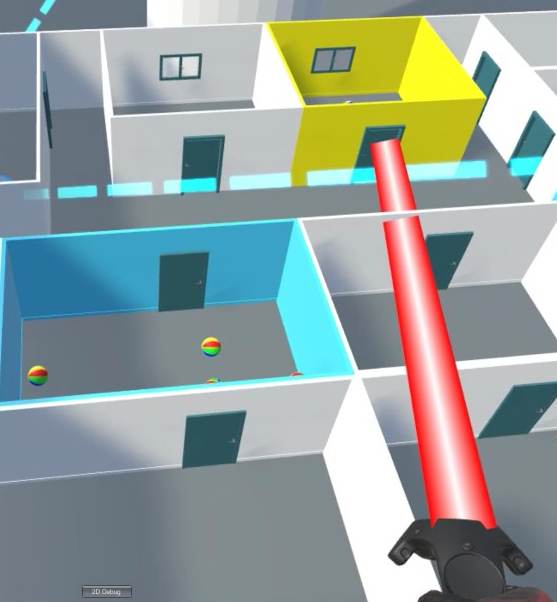
\includegraphics[height=6cm]{figures/screenshots/laserpointer}
    \caption{Mit dem Laserpointer wird ein Raum anvisiert.}
    \label{fig:laserpointer_screenshot}    
\end{figure}

Wie im vorigen Abschnitt beschrieben findet die Interaktion zwischen Vive-Controller und einem Raum statt, wenn der Controller den Raum überlappt.
Da jedoch beim Laserpointer der Controller vom Raum entfernt ist, muss hier eine Modifikation vorgenommen werden.
Intern nutzt das SteamVR-\lstinline|Hand|-Skript (welches den Controller repräsentiert und trackt) die Felder \lstinline|HoverSphereTransform| und \lstinline|HoverSphereRadius|.
Beide Felder definieren eine unsichtbare Kugel mit einem gegebenen Radius.
Standardmäßig folgt diese Kugel der Position des Controllers.
Sobald die Kugel mit einem \lstinline|Interactable|-Objekt überlappt, werden die entsprechenden SteamVR-Events ausgelöst.
Für den Laserpointer wird diese Kugel verschoben, wenn der Raycast einen Schnittpunkt mit einem auswählbaren Raum ergibt.
Die Position der Kugel wird auf den Schnittpunkt geändert, wodurch sie sich effektiv am Ende des Laserstrahls befindet.
Damit werden die SteamVR-Events für den entsprechenden Raum am Ende des Strahls ausgelöst.
\autoref{fig:laserpointer_sketch} verdeutlicht diesen Vorgang.
Wenn der Raycast keinen Schnittpunkt mit einem auswählbaren Raum ergibt, wird die Kugel wieder auf die Controller-Position zurückgesetzt.
\begin{figure}[hbt]
    \centering
    \begin{subfigure}{0.5\linewidth}
        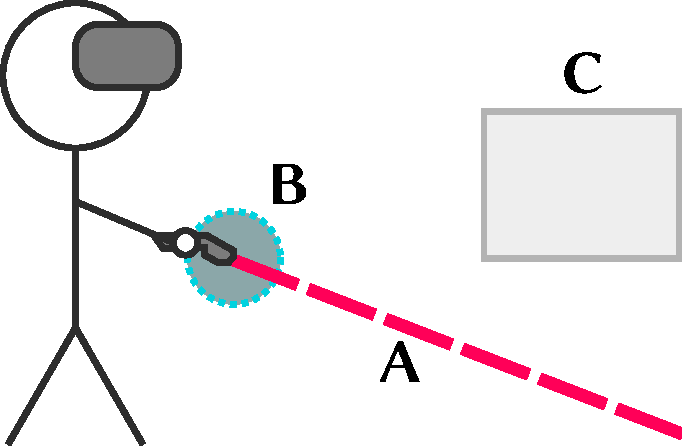
\includegraphics[width=\linewidth]{figures/laserpointer_sketch_no_hit}
        \caption{}
        \label{sfig:laserpointer_sketch_no_hit}
    \end{subfigure}%
    \begin{subfigure}{0.5\linewidth}
        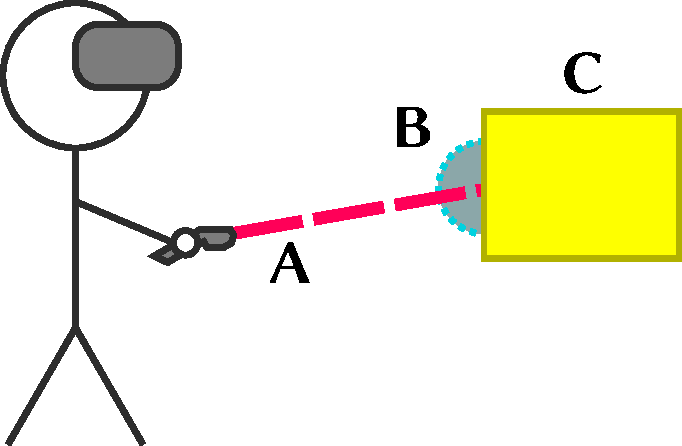
\includegraphics[width=\linewidth]{figures/laserpointer_sketch_hit}
        \caption{}
        \label{sfig:laserpointer_sketch_hit}
    \end{subfigure}
    \caption{Funktionsweise des Laserpointers. %
        Die \lstinline|HoverSphere| wird verschoben, sodass der Raum auf den Vive-Controller reagiert. %
        \textbf{A:} Laserpointer. \textbf{B:} SteamVR-\lstinline|HoverSphere|. \textbf{C:} Auswählbarer Raum.}
    \label{fig:laserpointer_sketch}
\end{figure}

%
\cleardoublepage
